
\documentclass[11pt]{article}
% ------- TikZ Guide Lines -------
\newcommand{\SSTGuidesPoints}[2]{% #1=basename (e.g. P), #2=last index
  \ifsstguides
    \foreach \i in {1,...,#2}{
      \fill[blue] (#1\i) circle (1.2pt);
      \node[blue,font=\scriptsize,above] at (#1\i) {\i};
    }
    \draw[gray!40, dashed]
    \foreach \i [remember=\i as \lasti (initially 1)] in {2,...,#2,1} { (#1\lasti)--(#1\i) };
  \fi
}
% ------- TikZ Guide Lines -------

% ------- TikZ Preamble -------
\RequirePackage{tikz}
\usetikzlibrary{knots,hobby,calc,arrows.meta,intersections,decorations.pathreplacing,decorations.markings,shapes.geometric,spath3}
\usepackage{amsmath}
\usepackage{hyperref}
\usepackage{calc,pict2e}
% stix replaces amssymb/amsfonts; loading both exceeds the symbol-font limit ("Too many symbol fonts declared").
\usepackage{stix}




% Document
\begin{document}


    \begin{tikzpicture}
        \path[spath/save=trefoil]
        (0,2) .. controls +(2.2,0) and +(120:-2.2) ..
        (210:2) .. controls +(120:2.2) and +(60:2.2) ..
        (-30:2) .. controls +(60:-2.2) and +(-2.2,0) .. (0,2);
        \tikzset{
          every trefoil component/.style={draw},
          spath/knot={trefoil}{15pt}{1,3,5},
        }
    \end{tikzpicture}


    \begin{tikzpicture}
        \path[spath/save=trefoil]
        (0,2) .. controls +(2.2,0) and +(120:-2.2) ..
        (210:2) .. controls +(120:2.2) and +(60:2.2) ..
        (-30:2) .. controls +(60:-2.2) and +(-2.2,0) .. (0,2);
        \tikzset{
          every trefoil component/.style={draw},
          spath/draft mode=true,
          spath/knot={trefoil}{15pt}{1,3,5},
          spath/get components of={trefoil}\cpts
        }
        \foreach[count=\k] \cpt in \cpts {
          \node[fill=white] at (spath cs:{\cpt} .5) {\k};
        }
    \end{tikzpicture}

    \begin{tikzpicture}
        \path[spath/save=trefoil]
        (0,2) .. controls +(2.2,0) and +(120:-2.2) ..
        (210:2) .. controls +(120:2.2) and +(60:2.2) ..
        (-30:2) .. controls +(60:-2.2) and +(-2.2,0) .. (0,2);
        \tikzset{
          every trefoil component/.style={draw},
          trefoil component 1/.style={blue},
          trefoil component 2/.style={green, dashed, |<->|},
          trefoil component 3/.style={magenta, line width=2pt},
          spath/knot={trefoil}{15pt}{1,3,5},
        }
    \end{tikzpicture}

% --- 3₁ Half-Twist Trefoil ---
    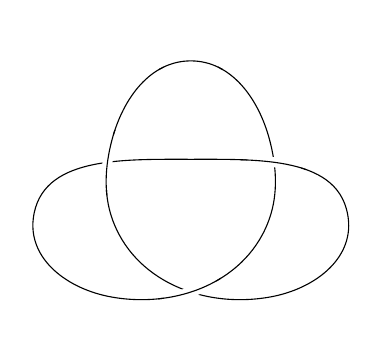
\begin{tikzpicture}[use Hobby shortcut]
        \coordinate (P1) at (0.0, 2.0);
        \coordinate (P2) at (-1.0, 1.0);
        \coordinate (P3) at (-1.0, 0.0);
        \coordinate (P4) at (1.0, -1.0);
        \coordinate (P5) at (2.0, 0.0);
        \coordinate (P6) at (0.0, 0.75);
        \coordinate (P7) at (-2.0, 0.0);
        \coordinate (P8) at (-1.0, -1.0);
        \coordinate (P9) at (1.0, 0.0);
        \coordinate (P10) at (1.0, 1.0);

        \begin{knot}[
            consider self intersections=true,
            ignore endpoint intersections=false,
            flip crossing/.list={2,4,6,8,10,12,14},
        ]
            \strand ([closed] P1)..(P2)..(P3)..(P4)..(P5)..(P6)..(P7)..(P8)..(P9)..(P10);
        \end{knot}
    \end{tikzpicture}



    % --- 5₁ Torus Cinquefoil ---

    \begin{tikzpicture}
        \begin{knot}[
          consider self intersections=true,
          draft mode=crossings,
          flip crossing=2,
          only when rendering/.style={show curve controls}
          ]
        \strand (0,2) .. controls +(2.2,0) and +(120:-2.2) .. (210:2) .. controls +(120:2.2) and +(60:2.2) .. (-30:2) .. controls +(60:-2.2) and +(-2.2,0) .. (0,2);
        \end{knot}
    \end{tikzpicture}



    \begin{tikzpicture}
        \begin{knot}[
          consider self intersections=true,
          draft mode=crossings,
          flip crossing/.list={2,4},
          only when rendering/.style={show curve controls}
        ]
        \strand (2,0) .. controls +(0,1.0) and +(54:1.0) .. (144:2) .. controls +(54:-1.0) and +(18:-1.0) .. (-72:2) .. controls +(18:1.0) and +(162:-1.0) .. (72:2) .. controls +(162:1.0) and +(126:1.0) .. (-144:2) .. controls +(126:-1.0) and +(0,-1.0) .. (2,0);
        \end{knot}
    \end{tikzpicture}



% --- 7₁ Torus Septafoil ---
    \begin{tikzpicture}[use Hobby shortcut]
        \coordinate (P1) at (-0.25, 2.0);
        \coordinate (P2) at (-1.50, 0.50);
        \coordinate (P3) at (-1.50, 0.0);
        \coordinate (P4) at (0.50, -1.0);
        \coordinate (P5) at (1.0, -0.75);
        \coordinate (P6) at (1.25, 1.25);
        \coordinate (P7) at (0.75, 1.75);
        \coordinate (P8) at (-0.75, 1.75);
        \coordinate (P9) at (-1.25, 1.25);
        \coordinate (P10) at (-1.0, -0.75);
        \coordinate (P11) at (-0.50, -1.0);
        \coordinate (P12) at (1.50, 0.0);
        \coordinate (P13) at (1.50, 0.50);
        \coordinate (P14) at (0.25, 2.0);
        \coordinate (P15) at (-0.25, 2.0);
        \begin{knot}[
            consider self intersections,
            ignore endpoint intersections=false,
            flip crossing/.list={2,4,6,8,10,12,14,16,18},
        ]
            \strand ([closed] P1)..(P2)..(P3)..(P4)..(P5)..(P6)..(P7)..(P8)..(P9)..(P10)..(P11)..(P12)..(P13)..(P14)..(P15);
        \end{knot}
    \end{tikzpicture}


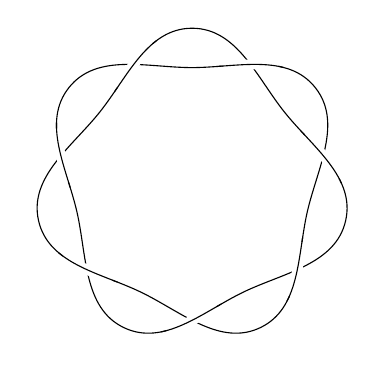
\begin{tikzpicture}[use Hobby shortcut]
    \begin{knot}[
      consider self intersections=true,
    %  draft mode=crossings,
      flip crossing/.list={2,4,6}
    ]
        \strand ([closed]90:2) foreach \k in {1,...,7} { .. (90-360/7+\k*720/7:1.5) .. (90+\k*720/7:2) } (90:2);
    \end{knot}
\end{tikzpicture}


% --- 9₁ Torus Nonafoil (alt) ---
    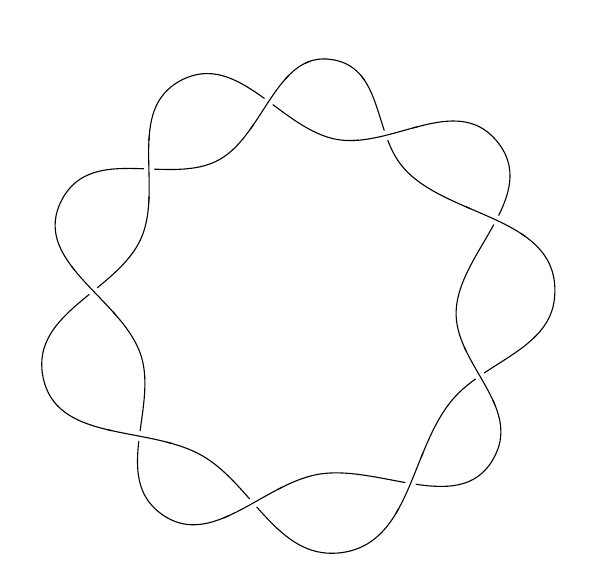
\begin{tikzpicture}[use Hobby shortcut]
        \coordinate (P1) at (0.25, 3.25);
        \coordinate (P2) at (-1.25, 2.0);
        \coordinate (P3) at (-3.25, 1.50);
        \coordinate (P4) at (-2.25, -0.50);
        \coordinate (P5) at (-2.0, -2.50);
        \coordinate (P6) at (0.0, -2.0);
        \coordinate (P7) at (2.25, -1.75);
        \coordinate (P8) at (1.75, 0.0);
        \coordinate (P9) at (2.25, 2.25);
        \coordinate (P10) at (0.25, 2.25);
        \coordinate (P11) at (-1.75, 3.0);
        \coordinate (P12) at (-2.25, 1.0);
        \coordinate (P13) at (-3.50, -0.75);
        \coordinate (P14) at (-1.50, -1.75);
        \coordinate (P15) at (0.25, -3.0);
        \coordinate (P16) at (1.75, -1.0);
        \coordinate (P17) at (3.0, 0.25);
        \coordinate (P18) at (1.0, 2.0);
        \begin{knot}[
            consider self intersections,
            ignore endpoint intersections=false,
            flip crossing/.list={2,4,6,8,10,12,14,16,18,20},
        ]
            \strand ([closed] P1)..(P2)..(P3)..(P4)..(P5)..(P6)..(P7)..(P8)..(P9)..(P10)..(P11)..(P12)..(P13)..(P14)..(P15)..(P16)..(P17)..(P18);
        \end{knot}
    \end{tikzpicture}


\end{document}